% CHAPITRE 3
\chapter{Bilan de C de la tourbière de La Guette}
\newpage

\section{Introduction}

\section{Matériels et méthodes}

\subsection{méthodes de mesure}

\subsubsection{mesures de flux de gaz}
La mesure des flux de \coo et de \chh ont été effectué en utilisant la méthode décrite dans la partie~\ref{sec:clsd_chbr_method}.
En XmoisX YannéeY, 20 placettes ont été installées\footnote{je remercie ici Sébastien Gogo pour avoir installé ces placettes sur le terrain avant même mon arrivée.}. 
Les placettes délimitées par des piquets occupaient une surface de \SI{4}{\square\metre} (2$\times$\SI{2}{\metre}), à l'intérieur de laquelle ont été installé de façon permanente un piézomètre et une embase permettant la mesure des flux de gaz.
Usuellement des placettes sont séparées en groupes micro-topographique ce qui à l'avantage de permettre une distinction des capacités sources/puits relativement fine mais qui à généralement l'inconvénient du placement proche des embases les unes des autres.
Afin de gagner en représentativité spatiale, la taille du site le permettant, il a été décidé de positionner des placettes sur l'ensemble du site selon un échantillonnage aléatoire stratifié.
De plus, du fait de l'omniprésence de végétation vasculaire, et de la taille des chambres par rapport à la micro-topographie une telle approche était difficile à mettre en oeuvre.

Les mesures de \coo ont été effectué de mars 2013 à février 2015, avec une fréquence quasiment mensuelle (20 campagnes, pour 24 mois de mesure).

Les mesures de \chh ont été effectuées avec une fréquence moindre principalement liée au difficulté de mise en oeuvre de l'instrument SPIRIT (lourd, difficilement transportable dans un milieu tourbeux).

\subsubsection{Les facteurs contrôlants}

Les mesures manuelle effectuées sont la mesure de la pression atmosphérique, du PAR, des températures du sol à différentes profondeur, de la végétation.

Les mesures automatiquement acquise via une station météo campbell sont la température de l'air, température de la tourbe à X, X et X profondeur, vitesse et direction du vent, humidité relative de l'air, irradiation solaire, pression atmosphérique.

\subsection{modélisation du bilan de C}

Afin de pouvoir interpoler les mesures de respiration mensuelles, il est nécessaire de les relier à des variables environnementales nous l'avons vu.
Un des facteurs de contrôle des flux est la température qui régule les processus chimiques et biologiques.
La température à \SI{-5}{\cm} est la plus souvent utilisée \cite{ballantyne2014}, même si d'autres comme la température de l'air ou encore la température du sol à \SI{-10}{\cm} peuvent également l'être \cite{bortoluzzi2006,kim1992}.
Cette profondeur, \SI{-5}{\cm}, est régulièrement utilisée car c'est dans la tourbe, proche de la surface qu'est produit la majorité du \coo.
\textbf{production CO2 ? profils ?}
C'est également à des profondeurs relativement faibles que se situent la majorité des racines \plop qui peuvent contribuer à la respiration du sol \textbf{(de l'écosystème?)} pour 35 à \SI{60}{\percent} \cite{silvola1996a,crow2005}.

\section{Évolution générale des facteurs contrôlants et des flux}

\subsection{Les facteurs contrôlants}

L'évolution du niveau de la nappe des 20 placettes, décrite dans la figure~\ref{fig:WTL_mean_evolution}, est marquée par un étiage d'une vingtaine de centimètres en moyenne en 2013 et l'absence d'un étiage net en 2014 avec un niveau de la nappe moyen ne descendant que rarement sous la barre des \SI{-10}{\cm}.
Ces observations sont cohérentes avec la figure~\ref{fig:WTL} représentant des données acquises à plus haute fréquence, et confirment la particularité de ces 2 années vis à vis des précédentes qui présentent des étiages bien plus fort.

\begin{figure}
\centering
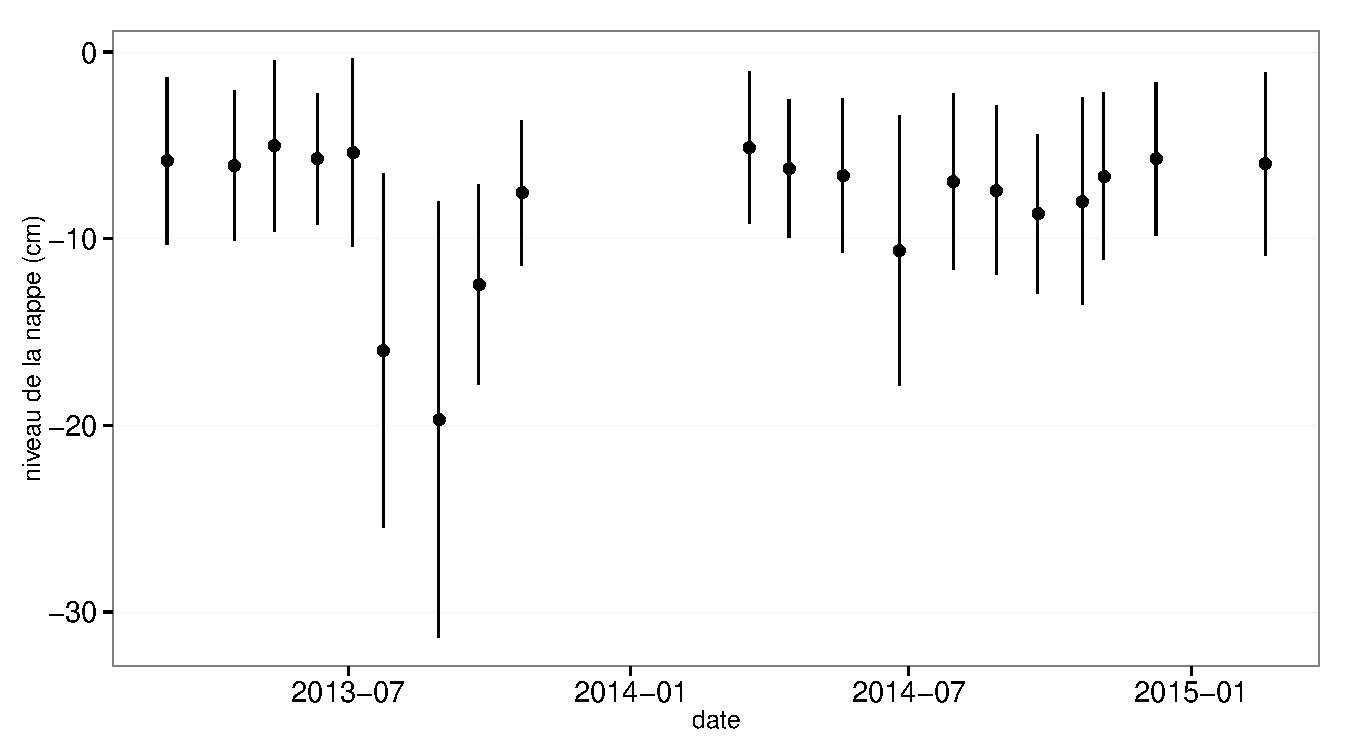
\includegraphics[width=\textwidth]{chap3/WTL_mean_evolution}
\caption{Évolution du niveau de la nappe moyen des 20 embases pendant la période de mesure (mars 2013 -- février 2015)}
\label{fig:WTL_mean_evolution}
\end{figure}


\begin{figure}
\centering
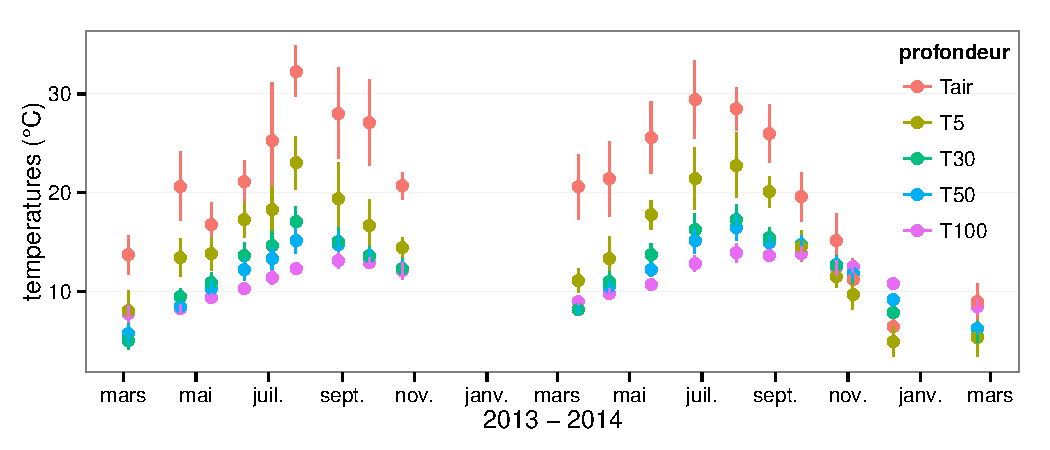
\includegraphics[width=\textwidth]{chap3/T_mean_evolution}
\caption{Évolution des températures pendant la période de mesure (mars 2013 -- février 2015)}
\label{fig:T_mean_evolution}
\end{figure}


\begin{figure}
\centering
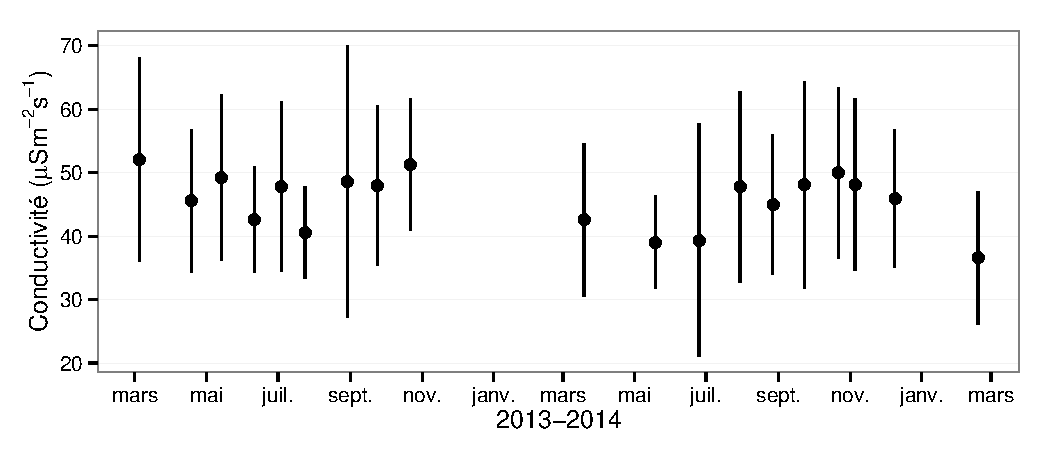
\includegraphics[width=\textwidth]{chap3/cond_mean_evolution}
\caption{Évolution de la conductivité pendant la période de mesure (mars 2013 -- février 2015)}
\label{fig:cond_mean_evolution}
\end{figure}

\begin{figure}
\centering
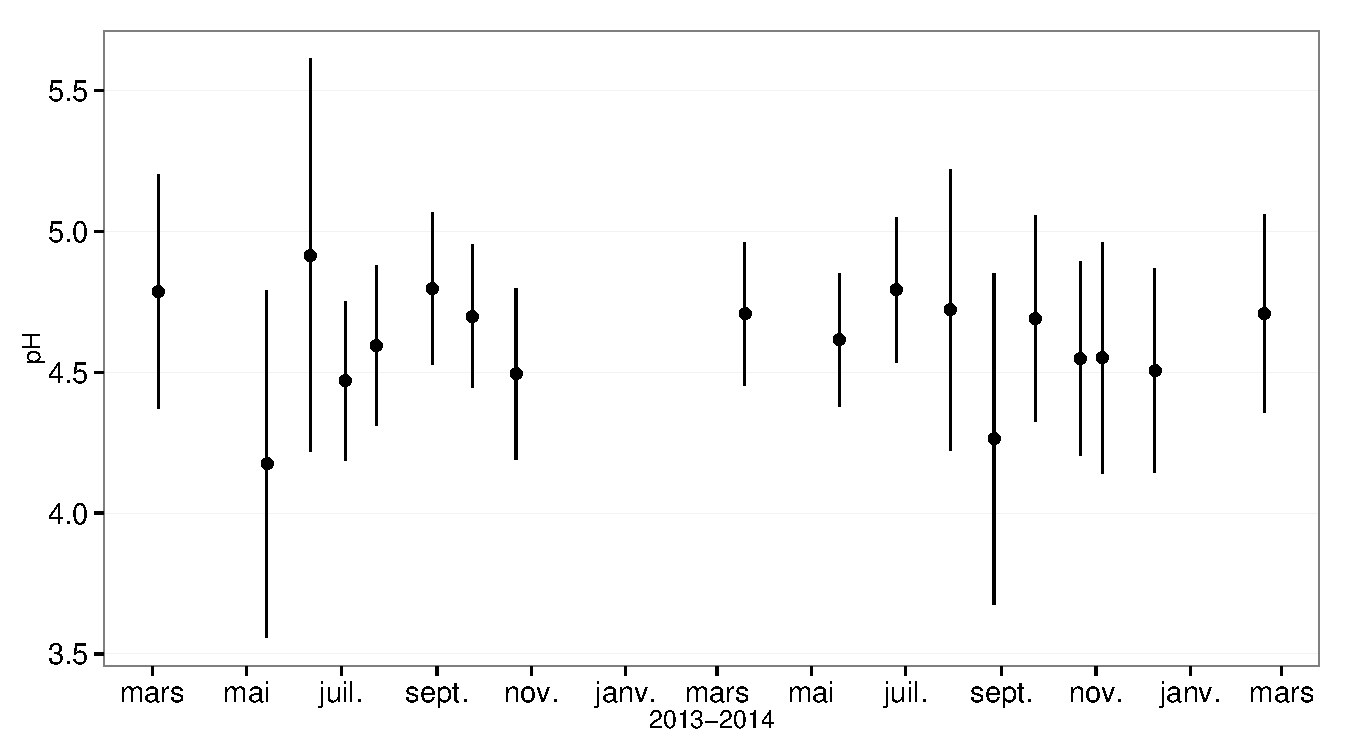
\includegraphics[width=\textwidth]{chap3/pH_mean_evolution}
\caption{Évolution du pH pendant la période de mesure (mars 2013 -- février 2015)}
\label{fig:pH_mean_evolution}
\end{figure}


\begin{figure}
\centering
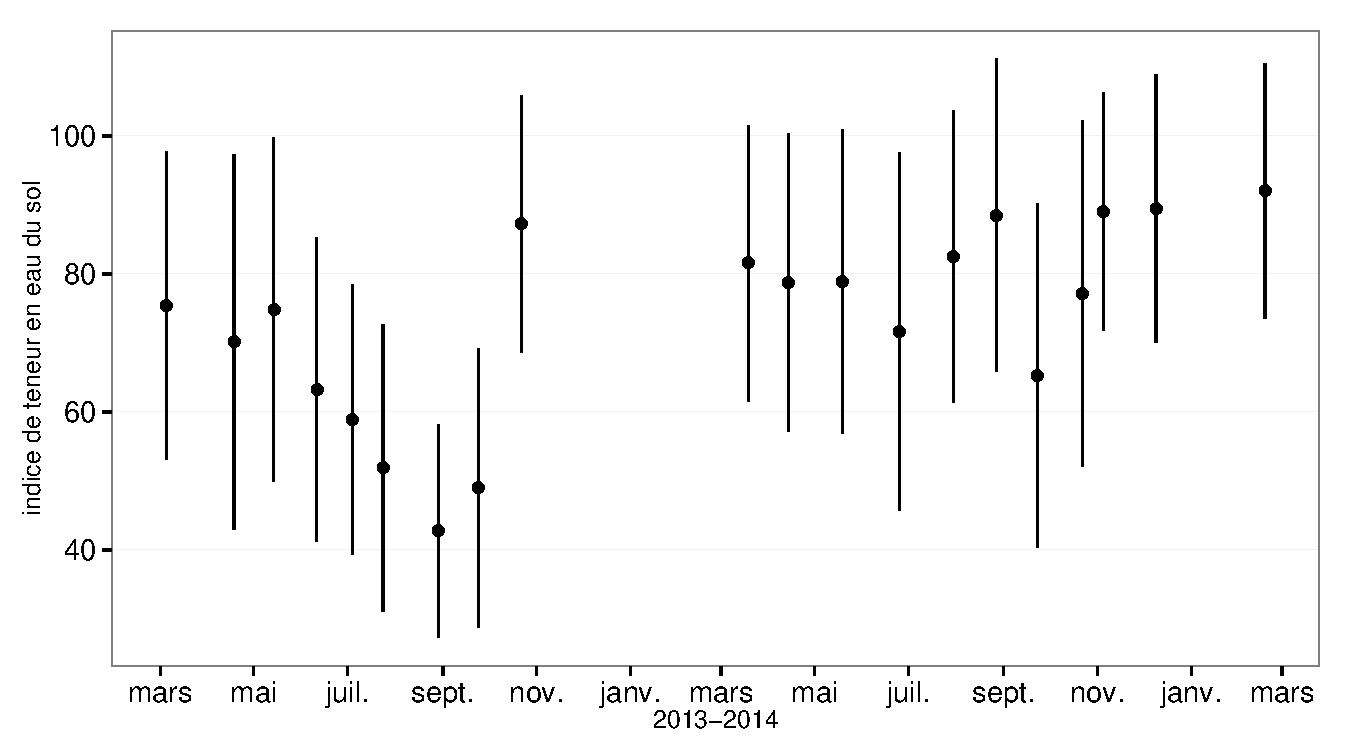
\includegraphics[width=\textwidth]{chap3/RH_mean_evolution}
\caption{Évolution de la teneur en eau du sol pendant la période de mesure (mars 2013 -- février 2015)}
\label{fig:RH_mean_evolution}
\end{figure}
\subsection{Le \coo}


\begin{figure}
	\centering
	\begin{subfigure}[t]{\textwidth}
		\centering
		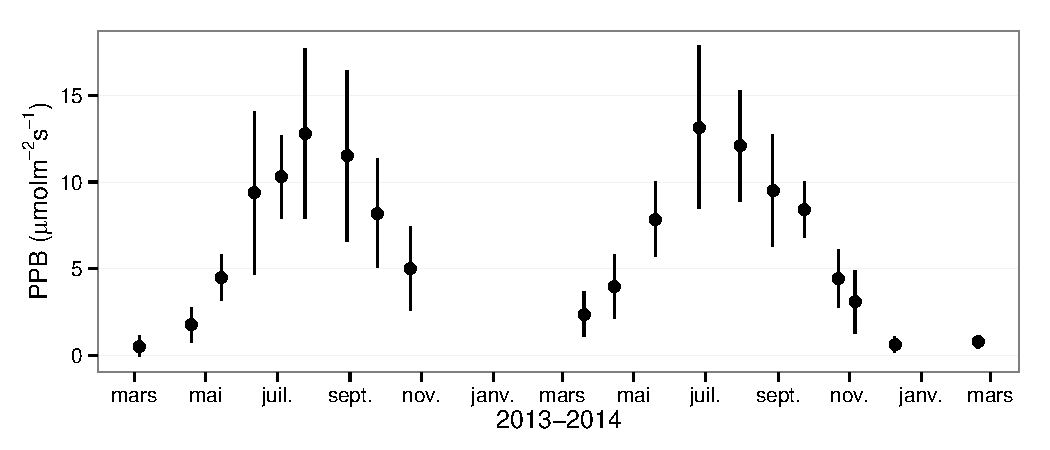
\includegraphics[width=\textwidth]{chap3/GPP_evolution_avg}
		\caption{Production primaire brute}
		\label{fig:GPP_evolution_avg}
	\end{subfigure}%
	
	\begin{subfigure}[t]{\textwidth}
		\centering
		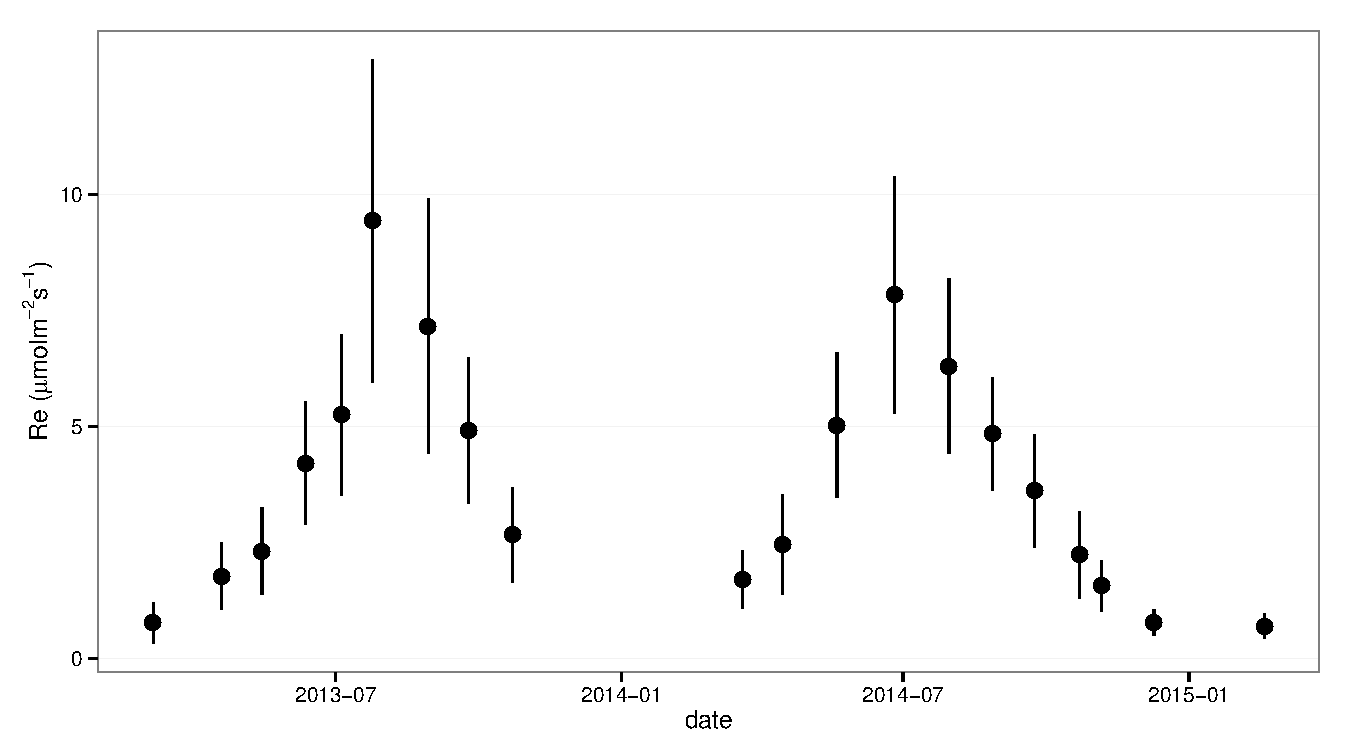
\includegraphics[width=\textwidth]{chap3/ER_evolution_avg}
		\caption{Respiration de l'écosystème}
		\label{fig:ER_evolution_avg}
	\end{subfigure}
	
	\begin{subfigure}[t]{\textwidth}
		\centering
		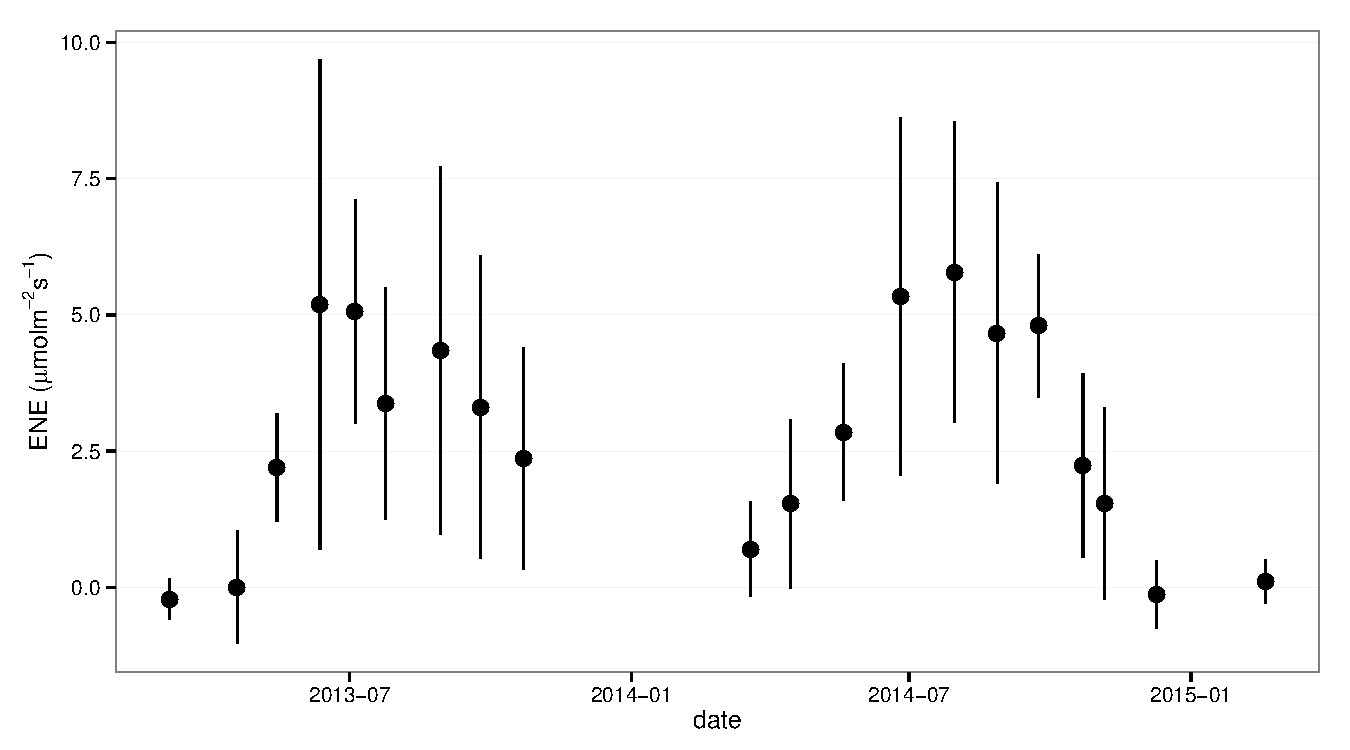
\includegraphics[width=\textwidth]{chap3/NEE_evolution_avg}
		\caption{Échange net de l'écosystème}
		\label{fig:NEE_evolution_avg}
	\end{subfigure}
\caption{Évolution du niveau de PPB, RE et ENE pendant la période de mesure. Moyenne des 20 embases de mars 2013 à février 2015.}
\label{fig:flux_evolution_avg}
\end{figure}

%\subsubsection{PBB}
L'ensemble des mesures de \coo s'étendent de mars 2013 à février 2015.
Cependant de novembre 2013 à février 2014 les mesures ont été interrompue suite à des pannes/casses matérielles.
Malgré cela les périodes les plus critiques, notamment la saison de végétation, ont pu être mesurées pour les 2 années, permettant d'avoir une vision correcte/globale de chacune d'elle.
À noter également que pour l'ensemble des flux, la déviation standard augmente avec les valeurs mesurées.

En 2013, les valeurs de la PPB augmentent au printemps et une partie de l'été avec un maximum de \SI{999999(888)}{\uml} atteint fin juillet, avant de diminuer à partir d'août.
En 2014 le maximum de PPB, \SI{99999(888)}{\uml}, est atteint en juin, soit plus tôt que l'année précédente.
Puis pendant l'été et l'automne les valeurs décroissent jusqu'à être proche de 0.
En moyenne les valeurs de la PPB sont de \SI{7.12(519)}{\uml} en 2013 et de \SI{6.56(472)}{\uml} en 2014 (Figure~\ref{fig:GPP_evolution_avg}).


%\begin{figure}
%\centering
%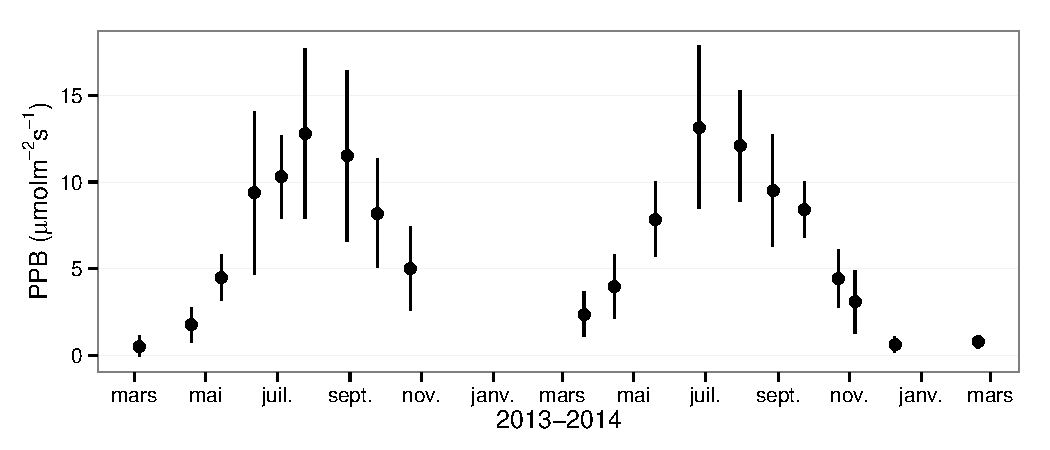
\includegraphics[width=\textwidth]{chap3/GPP_evolution_avg}
%\caption{Évolution du niveau de la production primaire brute, moyenne des 20 embases pendant la période de mesure (mars 2013 -- février 2015)}
%\label{fig:GPP_evolution_avg}
%\end{figure}

%\subsubsection{ER}

La RE en 2013 augmente pendant le printemps et une partie de l'été, elle atteint un maximum de \SI{99999(888)}{\uml} en juillet avant de diminuer.
En 2014 la RE atteint, comme la PPB, son maximum plus tôt, en juin à \SI{99999(888)}{\uml} avant de décroître jusqu'en hiver pour approcher des valeurs nulles.
La moyenne annuelle de RE en 2013 est de \SI{4.27(316)}{\uml}, ce qui est légèrement supérieure à celle de 2014 : \SI{3.63(256)}{\uml}(Figure~\ref{fig:ER_evolution_avg}).



%\begin{figure}
%\centering
%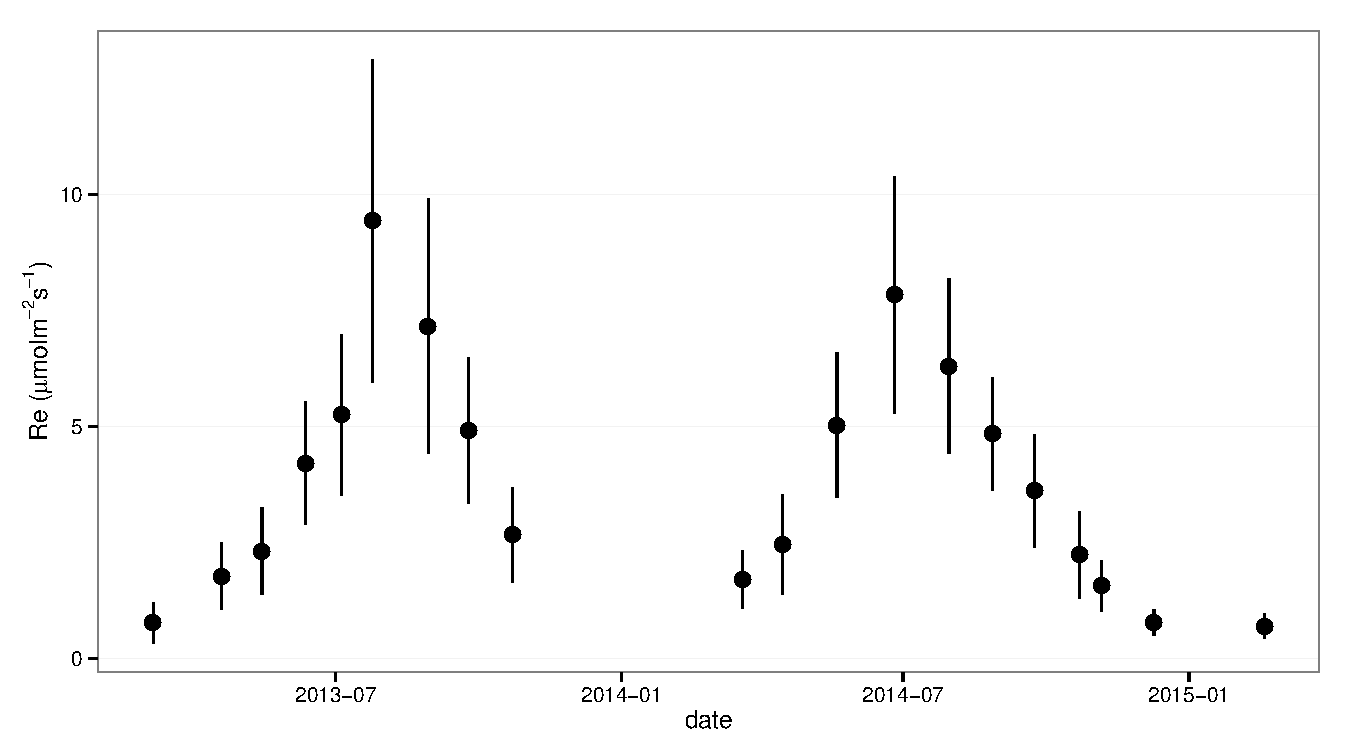
\includegraphics[width=\textwidth]{chap3/ER_evolution_avg}
%\caption{Évolution du niveau de la respiration de l'écosystème, moyenne des 20 embases pendant la période de mesure (mars 2013 -- février 2015)}
%\label{fig:ER_evolution_avg}
%\end{figure}

%\subsubsection{ENE}

Concernant l'ENE, en 2013 elle augmente jusqu'en juin avec un maximum à \SI{99999(888)}{\uml} avant de diminuer jusqu'à la fin de l'année.
Cependant, cette baisse est moins homogène que celle des deux flux précédents, avec notamment une augmentation de l'ENE entre juillet et août 2013.
Ceci étant, il faut également noter les valeurs importantes de la déviation standard particulièrement en juin et en août.
En 2014, l'ENE maximum est atteinte en juillet avec \SI{99999(888)}{\uml} avant qu'elle ne décroisse.
Cette baisse est cependant plus homogène qu'en 2013.
les moyennes de l'ENE en 2013 et 2014 sont très proche est sont respectivement de \SI{2.85(305)}{\uml} et \SI{2.93(277)}{\uml} (Figure~\ref{fig:NEE_evolution_avg}).



%\begin{figure}
%\centering
%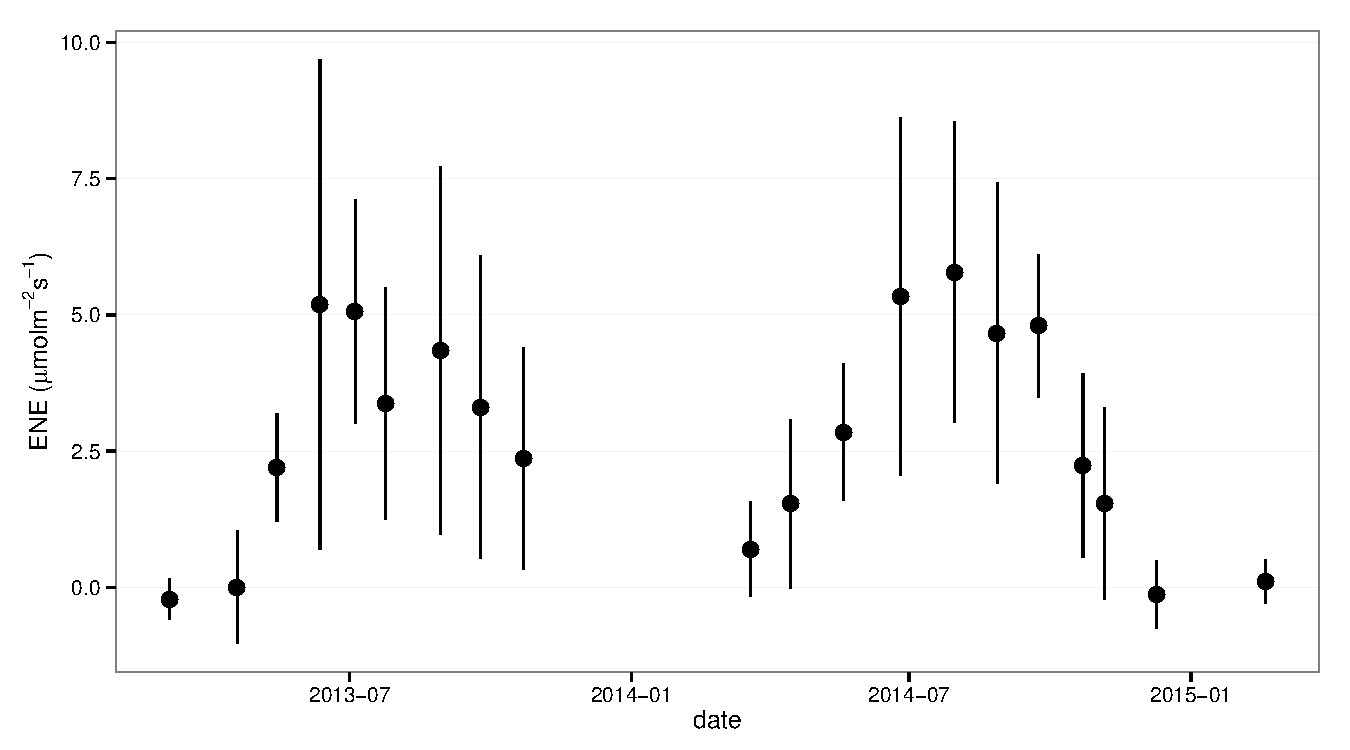
\includegraphics[width=\textwidth]{chap3/NEE_evolution_avg}
%\caption{Évolution du niveau de l'échange net de l'écosystème, moyenne des 20 embases pendant la période de mesure (mars 2013 -- février 2015)}
%\label{fig:NEE_evolution_avg}
%\end{figure}

\subsection{Le \chh}

\begin{figure}
\centering
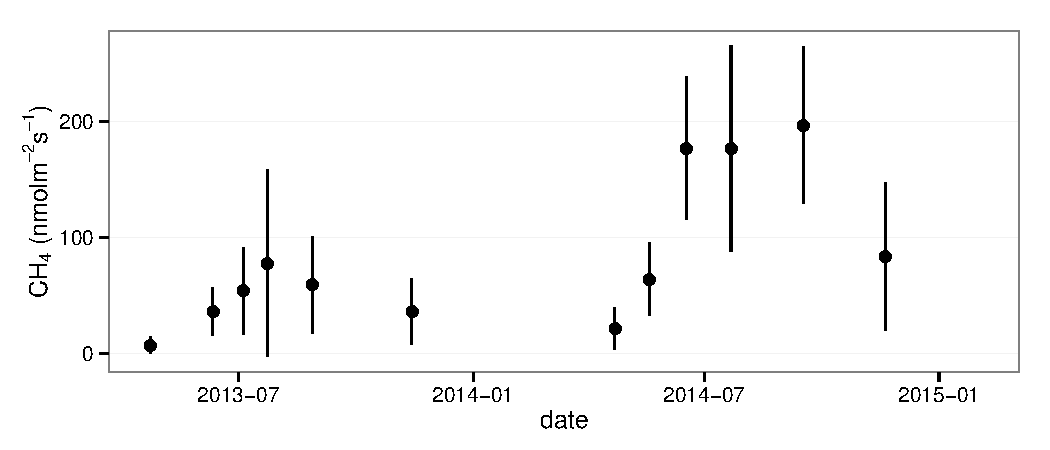
\includegraphics[width=\textwidth]{chap3/CH4_evolution_avg}
\caption{Évolution des flux de méthane moyen (N ?) pendant la période de mesure (mars 2013 -- février 2015)}
\label{fig:CH4_evolution_avg}
\end{figure}

\subsection{Le Carbone Organique Dissous (COD)}

\section{Le bilan de carbone}

\begin{align}
RE &= a \times exp(b\times T5)\\
PPBsat &= a \times exp(-((Tair - b)/ c)^2)\\
ENE &= PPB - RE\\
ENE &= a \times exp(b\times T5) - a \times exp(-((Tair - b)/ c)^2)
\end{align}
\section{Évaluation du bilan}

\subsection{sensibilité des paramètres}

\subsection{capacité à modéliser d'autres données}

\subsection{représentativité locale}

\section{représentativité locale ?}